\documentclass[12pt]{article}
\usepackage{graphicx}
\def\baselinestretch{1.5}
\setlength{\topmargin}{0pt}
\setlength{\textheight}{570pt}
\setlength{\oddsidemargin}{0pt}
\setlength{\evensidemargin}{60pt}
\setlength{\textwidth}{427pt}
%\setlength{\footheight}{0pt}
\setlength{\footskip}{30pt}
\parindent 25pt
\hyphenpenalty=10000
\tolerance=10000
\pagestyle{plain}

\begin{document}
\begin{flushleft}

Estimating effective population size and mutation rate from sequence data using 
Metropolis-Hastings sampling

\bigskip
\bigskip
Mary K. Kuhner$^*$, Jon Yamato, and Joseph Felsenstein$^{\dag}$

Department of Genetics, University of Washington

Seattle, WA 98195, USA

\bigskip
$^*$Internet address {\it mkkuhner@genetics.washington.edu}

$^{\dag}$Internet address {\it joe@genetics.washington.edu}

\newpage
Running head:  Metropolis-Hastings sampling

\bigskip
Corresponding author:  
\bigskip

Mary K. Kuhner

Department of Genetics SK-50

University of Washington

Seattle, WA 98195, USA

Phone (206) 543-8751

FAX (206) 543-0754

Internet 
\begin{it}
mkkuhner@genetics.washington.edu
\end{it}

\newpage

\end{flushleft}
\begin{center}
ABSTRACT
\bigskip
\end{center}

We present a new way to make a maximum likelihood estimate of the parameter 
$4N_{e}\mu$ (effective
population size times mutation rate per site, or $\Theta$) based on a population 
sample of
molecular sequences.  We use a Metropolis-Hastings Markov chain Monte
Carlo method to
sample genealogies in proportion to the product of their likelihood with
respect to the data and their prior probability with respect to a
coalescent distribution.  A specific value of $\Theta$ must be chosen in
order to
generate the coalescent distribution, but the resulting trees can be
used to evaluate the likelihood at other values of $\Theta$,
generating a likelihood curve.  This
procedure concentrates sampling on those genealogies
which contribute most of the likelihood, allowing estimation of
meaningful likelihood curves based on relatively small samples.
The method can potentially be extended
to cases involving varying population size, recombination, and migration.

\bigskip
\begin{center}
INTRODUCTION
\end{center}

\bigskip
The genealogy representing the relationship between a set of
gene copies randomly chosen from a population can be thought of as a
series of coalescences --- points at which two lineages had a common
ancestor (see Figure 1).  The time intervals between one coalescence and the next are
expected to have a distribution which depends on the
effective population size $4N_{e}$ (in a diploid population;
this paper will assume diploids, but the method is identical when
applied to haploids, with $4N_e$ replaced by $2N_e$, and to
mitochondria, with $4N_e$ replaced by $2N_f$). 
In the absence of an outside
standard, molecular sequence data cannot give information on the actual
durations of these intervals, but only on the amount of change that occured
during them.  Therefore, instead of estimating $4N_{e}$ we must estimate its
product with the neutral mutation rate $\mu$.
This paper discusses a new method for estimating the
product $4N_{e}\mu$, also called $\Theta$, using sequence data taken from a
random sample of individuals from a population.

We wish to use the relationship between the intervals in the
genealogy and $\Theta$ to make a maximum likelihood estimate
of $\Theta$ from genealogies inferred from a population 
sample (for example, of nucleotide sequences).
An earlier paper ({\sc Felsenstein} 1992b) approached this problem using
bootstrapping.  Since the true genealogy is generally unknown, we wish to
base the estimate on
a number of plausible genealogies, weighting each one according to
its plausibility.  {\sc Felsenstein} suggested bootstrap resampling the DNA 
data and using the genealogies reconstructed from each bootstrap sample to
estimate $\Theta$ --- arguing that this
resampling procedure effectively chooses genealogies in proportion to
their likelihood with respect to the data, which is equivalent (if a large 
number of samples are
taken) to weighting the genealogies by their
likelihood.  For reasons which will be discussed below, we now believe
this approach to be incorrect.

In the current paper we present a new method of sampling genealogies.
The strategy is Metropolis-Hastings sampling:
a repeated process of modifying a genealogy and accepting or rejecting
it in proportion to the ratio of its probability
to the probability of the previous genealogy, as described by {\sc Metropolis}
et al. (1953) and modified by {\sc Hastings} (1970). 
We present the method as it applies to DNA or RNA sequence data, but it
could readily be adapted to other types of information for which models
of the change process are available, such as restriction site data.
As presented, this method is appropriate for use in cases where
recombination does not occur, such as mitochondrial DNA, but we hope in the future
to extend it to cases involving recombination, migration, and varying
population size.

We would like to compute the likelihood of the observed sequence data for 
a given value of $\Theta$, $L(\Theta)$, in order to find the value of
$\Theta$ which maximizes the likelihood of the data, and to assess how
well supported this value is compared to others.  For a given genealogy, 
$L(\Theta)$ is the product
of the prior probability of the genealogy based on the coalescent distribution,
$P(G|\Theta)$, and the probability of the sequence data given the
genealogy, $P(D|G)$.  This product should be summed over all possible
genealogies to give the overall likelihood of the data set for a given
value of $\Theta$.
The prior probability has been described by {\sc Kingman} (1982a, b) and is
straightforward to calculate.  The probability of the sequence data for
a given genealogy is also readily computable ({\sc Felsenstein}
1981).  However, computation of the overall likelihood $L(\Theta)=\sum_{G}P(D|G)P(G|\Theta)$ 
demands a summation over a huge number of topologies, each with an
infinite number of possible branch lengths.

Rather than sampling all genealogies, we could consider making a random sample;
but in practice most genealogies are extremely implausible explanations
of the sequence data and therefore contribute almost no
information to the estimate.  In order to get an accurate estimate,
the random sample would have to be unmanageably large.  Therefore, we use an
importance sampling approach:  we concentrate sampling on those
genealogies which are plausible and therefore will contribute
substantially to the estimate of $\Theta$.  

To use this approach,
we need to choose a known distribution from which to sample.
One approach would be to sample with respect to
the coalescent prior $P(G|\Theta)$ --- the prior probability of a genealogy
at a given value of $\Theta$, without regard to the data.  This is easily 
done, but most of the genealogies drawn from $P(G|\Theta)$ do not 
contribute substantially to
the likelihood because their topology is implausible for the
given data, making this type of sampling very inefficient.

Another
approach would be to sample genealogies from a probability density
proportional to the probability of the data
given the genealogy, $P(D|G)$.
One of us ({\sc Felsenstein} 1992b) previously proposed to estimate $\Theta$
by bootstrapping:  that is, repeatedly making new data sets by
sampling with replacement from the original one, estimating the
genealogy from each new data set, and treating each of the resulting 
genealogies as an
independent sample from $P(D|G)$.  Only limited simulation of this method
was undertaken due to its slowness and to technical difficulties (when
the true value of 
$\Theta$ is small, some bootstrap replicate data sets contain no variable
sites, and such data sets disrupt the estimate).  These simulations
were not sufficient to establish whether or not this method (the bootstrap Monte
Carlo method) is unbiased.  We now know it to be biased, for the
following reason.

The bootstrap resampling is attempting to sample points from a
distribution proportional to $P(D|G)$.  This is not a legitimate
distribution to sample from:  it has infinite area.  Consider the case
of only two sequences, and suppose that the data provide no information
about the correct branch length back to their coalescence (for example,
zero bases were sampled).  In this
case, the branch length could take any value from zero to infinity with
equal probability, which means its expectation is infinitely large.
If the data provide some information, but not enough to establish the
branch length with perfect certainty, there will be an upwards bias in
the estimate of $\Theta$ because the space of longer trees to sample is
infinitely larger than the space of smaller trees, and longer
trees lead to a higher estimate of $\Theta$.
The proposal by {\sc Felsenstein} (1992b) to use Metropolis-Hastings
sampling based on $P(D|G)$ in place of bootstrapping has proven, when
implemented, to suffer from the same flaw, since it was sampling from
the same illegitimate distribution.

The practical consequence of sampling from this illegitimate
distribution is always an upward bias in the estimate of $\Theta$.  This
has been verified empirically by {\sc Richard Hudson} (pers. comm.) in simulations
evaluating the initially proposed form of the Metropolis-Hastings algorithm.  
{\sc Hudson's} simulations showed this
effect to be fairly severe with small data sets (200 bp from each of 20
individuals), with estimates two to three times higher than the true
value (data not shown).

Therefore, the strategy which we have chosen is to sample with respect to the
posterior probability of the genealogy, $P(D|G)P(G|\Theta)/P(D|\Theta)$, for a 
specific value of $\Theta$ which we will call $\Theta_{0}$.  (Although
the denominator $P(D|\Theta)$ is unknown, we need only compute the
ratio of the posterior probability for two genealogies, allowing this
term to be cancelled.)  To find the relative likelihood at other values of
$\Theta$ we divide through by the importance sampling function:

\begin{equation}
\frac{L(\Theta) }{L(\Theta_0)}
= \sum_{G} \left [ \frac{P(D|G)P(G|\Theta)}{P(D|G)P(G|\Theta_{0})}
\right ]
\end{equation}

Use of the posterior probability as an importance function allows us to sample 
genealogies which will 
make a substantial contribution to the eventual value of the likelihood, and
thus enables us to make a reasonable estimate of $\Theta$ by summing over a
finite number of genealogies.  It avoids the bias created by sampling
proportional to $P(D|G)$,
and practical experience suggests that it is much
less computationally intensive than the bootstrap approach.

\bigskip
\begin{center}
METHODS
\bigskip
\end{center}

\begin{bf}
Metropolis-Hastings Sampling:
\end{bf}
Our sampling strategy is to begin with an initial genealogy 
and make a small modification
to it,
choosing among a set of possible modifications according to their
relative probabilities based on the distribution $P(G|\Theta_0)$.
The probability of the data on the new genealogy ($P(D|G)$)
is then calculated, and compared with the probability on the
previous genealogy to decide whether or not the new genealogy should be
accepted.  If it is not, the old genealogy is retained.
  Repeating this process creates a Markov chain of genealogies
which, if run long enough, will travel among all genealogies in
proportion to their posterior probabilities $(P(D|G)P(G|\Theta)/P(D\Theta_0)$ 
for the given $\Theta_{0}$.

For the parameter $4N_e\mu$ we have chosen $\Theta$ rather
than $\theta$ as in other studies because we are measuring $\mu$ in terms
of mutations per site, not mutations per locus as in studies which use the
infinite-sites model.  Time is rescaled in terms of the mutation rate such
that in 1 unit of time the expected number of mutations per site is 1
(this simplifies use of the coalescent approximation).
We consider bifurcating, rooted, clocklike (ultrametric) genealogies.
Throughout this discussion, ``down'' is towards the root.
For ease of discussion, we will use the following convention:  a node's 
``parent'' is below it and its ``children'' are above it.  (In actuality
such a ``child'' represents a descendent of the ``parent'' a large
number of generations later, at the time of the next coalescence event.)

Figure 1 shows the modification process:
choosing a neighborhood (the region of the
genealogy to be changed), rearranging the
topology in that neighborhood, and choosing new branch lengths within the
neighborhood.  This is the fundamental operation of the algorithm, and
if applied repeatedly can transform any genealogy
into any other genealogy, thus allowing all possible genealogies to be
searched.
In practice, making larger rearrangements would probably make the sampling 
less efficient, because if a genealogy already has fairly high probability, a large
rearrangement of it is liable to be much worse, and therefore be
rejected.  However, such techniques may prove useful in analyzing very
large numbers of sequences, where the chance that the process will become
trapped in a local maximum of the posterior probability distribution is greater.

To make a rearrangement, a node is chosen at random from among all nodes 
which have both parents and children (i.e. are neither tips nor the
bottommost node of the genealogy).  This node will be referred to as the
``target''.  The neighborhood of rearrangement consists of the target node,
 its children,
parent, and parent's other child (see Figure 2A).  A rearrangement makes 
changes of two kinds:  it may reassort the three children among target and
parent, and it modifies the branch lengths within the neighborhood.
The new branch lengths must remain within the constraints imposed by the times
of the three children and of the parent's ancestor; these times define
the boundaries of the neighborhood.
Conceptually, the portion of the genealogy involving these nodes is erased
(see Figure 2B) and must now be redrawn.  The lineages to be erased and
redrawn will be referred to as ``active'' lineages, and the lineages existing
at the same time but outside the
neighborhood as ``inactive'' lineages.

To choose the times of the target and parent nodes, we draw from a
conditional coalescent
distribution with a given $\Theta$, which we call $\Theta_{0}$,
conditioned on the number of inactive lineages.  For
each time interval, the probability of coalescence among the active
lineages
depends on the numbers of active and inactive lineages present in the
genealogy during that interval.  A random walk, weighted by these
probabilities, is used to select a specific set of
times.  (This procedure is related to the Viterbi state-array algorithm
({\sc Viterbi} 1967) and is explained in detail in the Appendices.)
When the coalescence times have been determined, a topology compatible with
them is chosen at random (incompatible topologies are those in
which a child would be joined to a node whose branching time is above
the child's time).

Once the new genealogy is generated, the probability of the sequence
data on that genealogy is calculated under a
standard model ({\sc Felsenstein} 1981) much as is done in maximum likelihood
phylogeny estimation.  The Kimura
2-parameter model ({\sc Kimura} 1980) of sequence evolution, modified to 
allow unequal base frequencies ({\sc J. Felsenstein} unpublished,
described by {\sc Kishino} and {\sc Hasegawa} 1989),
is used to assess the probability of generating the observed data for
the given genealogy.  A different model could be
substituted in order to handle, for example, restriction site or amino
acid data; the rest of the method would be unchanged.

The objective of this algorithm is to create a Markov chain whose
states are genealogies, and whose
stationary probabilities are equal to the posterior probability 
$P(D|G)P(G|\Theta)/P(D|\Theta)$
of each genealogy.  {\sc Hastings} (1970) shows that this can be done using the
following relation, where $G$ is the old genealogy and $G'$ is the new:

\begin{equation}
r = 
\frac{P(D|G')}{P(D|G)} 
\frac{Q(G',G)}{Q(G,G')}
\end{equation}

$Q$ is the probability of generating the second
genealogy starting from the first under
the sampling strategy used.  In the simple form of
the Metropolis-Hastings algorithm presented here, the terms $Q(G',G)$
and $Q(G,G')$ are equal (they depend on the choice of target
node and of final topology, both of which have equal probabilities in either
direction) and therefore need not be calculated since their ratio is
always 1.  However, more complex versions of
the algorithm, such as those dealing with recombination, will probably
require calculation of the $Q$ terms.

If $r$ is greater than 1, the new genealogy is
accepted, replacing the old.  If it is less than 1, the new genealogy is
accepted with probability $r$; otherwise the old one is retained.

\bigskip

\begin{bf}
Computing the likelihood curve for $\Theta$: 
\end{bf}
At intervals, genealogies
created by this process can be sampled for use in constructing a
likelihood curve for $\Theta$.  (The question of how often to sample
will be touched on in the Discussion.)  The genealogies were produced
using importance sampling based on the known distribution $P(G|\Theta_0)$.
Computation of their likelihood under other values of $\Theta$ must 
therefore take this importance sampling function into account:

\begin{equation}
L(\Theta)=\sum_G \frac{P(D|G)P(G| \Theta)}{P(D|G)P(G| \Theta_0)}
\end{equation}

This equation can be reduced to a quickly calculatable form which
depends only on the structure of the genealogies:

\begin{equation}
L(\Theta)=\sum_G \frac{P(G| \Theta)}{P(G| \Theta_{0})}
\end{equation}

To compute the term $P(G|\Theta)$ (the prior probability of the
genealogy for the given $\Theta$), consider the
genealogy as a set of $i$ time intervals, each with length $t$ and number of
lineages $k$; the total number of tips is $n$.  The probability of the
genealogy is a product over all intervals ({\sc Kingman} 1982a, 1982b;
{\sc Felsenstein} 1992b):

\begin{Large}
\begin{equation}
P(G|\Theta)=\left (\frac{2}{\Theta}\right )^{n-1} \exp \left [{\sum
\limits_i \frac{-k(k-1)t_i}{\Theta}}\right ]
\end{equation}

\end{Large}

\medskip

A likelihood curve can be constructed using equation 3 for various
values of $\Theta$.  The maximum of this curve is a maximum likelihood
estimate of $\Theta$ and can be found by standard methods.  The curve is
not guaranteed to have a single maximum, but in practice we have found
that it generally does as long as the Markov chain has had sufficient
time to approach equilibrium.

\medskip

\begin{bf}
Combining multiple estimates:
\end{bf}
The closer the assumed value of $\Theta_{0}$ is to the true value of
$\Theta$, the more efficient this strategy becomes.  Therefore, it will often
be useful to repeat the Markov chain sampling several times, using the
estimate of $\Theta$ from each chain as the $\Theta_{0}$ of the next.
For maximum efficiency, the results of the earlier chains should not be
discarded, but combined with the results of the final chain to produce an
estimate of the overall likelihood curve, using an appropriate weighting.  The strategy
we use is due to {\sc Geyer} (1991) and treats the genealogies as having been
sampled from a mixture distribution of their various values of
$\Theta_0$.

Suppose that $m$ Markov chains have been run.
For a given run $j$, $n_{j}$ genealogies have been sampled, associated
with a given value of $\Theta_{0}$ which will be called $\Theta_{j}$. 
The overall $L(\Theta_{j})$
can be found by iterating the following relationship, where $\sum_{G}$
represents a summation over all of the sampled genealogies from all of
the Markov chains:

\begin{Large}
\begin{equation}
L(\Theta_{j})=\sum_{G} \frac{P(G|\Theta_{j})}
{\sum \limits_{i=1}^{m} \left ( n_{i} \frac{P(G|\Theta_{i})}{L(\Theta_{i})}
\right )}
\end{equation}
\end{Large}

When $\Theta_j$ is the $\Theta_0$ value at which one of the chains was
run, this is a nonlinear set of equations in the $L(\Theta_{j})$, which can
be solved iteratively by calculating new values of the $L(\Theta_{j})$
from the left hand side.  
Good starting values of the $L(\Theta_{i})$ can be obtained using the 
genealogies from the final Markov chain.  Likelihoods for other values
of $\Theta_j$ can then be interpolated using the same set of equations.

The likelihood curves produced by this approach are not guaranteed to be
unimodal, but in practice they usually are as long as enough iterations
were done to approach equilibrium.  We have found it best to run a
series of very short chains whose results are not used in the combined
estimate, in order for the genealogy and working value of $\Theta_0$ to
approach their final values.  Then a small number of much longer chains
can be used to make the final estimate.

\bigskip
\begin{center}RESULTS
\end{center}
\bigskip

{\bf Simulated data:}  We used computer simulation to explore the 
performance of this method.
Trees were constructed randomly according to the coalescent model, and DNA
sequence data evolved according to the 2-parameter model of {\sc Kimura} (1980)
using a transition/transversion ratio of 2.0. 
The UPGMA phylogeny reconstruction algorithm (as implemented in the PHYLIP
program NEIGHBOR v3.5) was used to construct
the starting tree to be used by the Metropolis-Hastings algorithm.
We investigated several parameters which could influence the performance
of the method:  length of sequence, number of individuals sampled, and
closeness of $\Theta_0$ to the true $\Theta$.
The simulations presented are far from exhaustive,
but can give a preliminary impression.

Table 1 shows results for samples of twenty individuals under three
conditions:  $\Theta_0$ ten times too low, equal to the true $\Theta$,
and ten times too high.  Results from the method of {\sc Watterson} (1975)
are provided for comparison.  In general, the two methods perform
about equally well.  The Metropolis-Hastings method shows little or no
bias towards $\Theta_0$.
This contrasts with runs in which only a single Markov chain was used,
in which a substantial bias towards $\Theta_0$ was seen (data not
shown).

Table 2 shows similar results for samples of 100 individuals.  Standard
deviations for the Metropolis-Hastings method are a little lower than
those for the method of Watterson.

Maximum likelihood methods in phylogenetics have typically been rather
computer intensive.
We timed our Metropolis-Hastings runs on a DECstation 5000/125 (a workstation of 
middling speed).  A representative entry from Table 2 (105,500 steps total along
the Markov chains) took 181.4 minutes. 
The majority of the runtime is consumed by likelihood calculations.
When a change is made, only the likelihoods for the nodes in the
neighborhood of rearrangement, and their ancestors down to the root of
the tree, need to be re-evaluated.  The mean number of such nodes
increases slowly with number of sequences, and therefore runtime is
not strongly dependent on number of sequences.
For a given number of iterations, runtime is expected to increase less than linearly with sequence
length, since identical sites are collapsed together during likelihood
calculation.  However, more iterations will be needed to adequately
search the space of plausible genealogies as the number of sequences
increases.

When Metropolis-Hastings and related algorithms fail to perform well, it
is generally because they become trapped in one part of their state
space and fail to sample other parts.  We have found it helpful to begin
with a UPGMA genealogy rather than a random genealogy to avoid wasting
time searching irrelevant parts of the genealogy space. 

{\bf Mitochondrial DNA sequence data:} 
{\sc Ward} et al. (1991) examined 360 bp from the
mitochrondial control region of 63 Amerindians of the Nuu-Chah-Nulth
tribe.  We analyzed both the full data set and two restricted data sets,
purine-only and pyrimidine-only (there are no sites with both purines
and pyrimidines in these data) in order to allow comparison with the
results of {\sc Tavar\'{e}} and {\sc Griffiths} (1993a). 
For the purine-only and pyrimidine-only data sets, base frequencies were
set at 0.49 for bases appearing in the data set and 0.01 for bases not
appearing; for the total data set they were calculated from the data.
The transition/transversion ratio was set to 100.0.   UPGMA was used to
generate initial trees for each data set separately.
The $\Theta$ estimate of {\sc Watterson} (1975) based on the 
number of segregating sites was used as the initial value for $\Theta_0$.
We did ten short runs of 1500 steps (sampling every tenth genealogy from the final
500 steps) and two long runs
of 12,000 steps (sampling every twentieth genealogy from the final
10,000 steps); the final estimate used only genealogies from the long runs.

For the full data the final estimate was 0.0396; the likelihood
curve is shown in Figure 3.  
(Note that in this case $\Theta=2N_f\mu$, where $N_f$ is the number of females,
since mtDNA is haploid and maternally inherited.)
This is substantially higher than the
estimate of 0.0153 produced by the method of {\sc Watterson} (1975) based on
counting the number of segregating sites; this difference is expected, 
since some of the sites in this data set have clearly had multiple
substitutions.
Purine sites alone produced an estimate of 0.00466 (Watterson estimate 
0.00667) and pyrimidine sites alone produced an estimate of 0.05237
(Watterson estimate 0.02217).  Proportionally more of the pyrimidine sites are
variable, suggesting that there may be a difference in mutation rate
between the two classes.  An appropriate extension of our method would
be to assign purine and pyrimidine sites to different mutation rate categories.

\bigskip
\begin{center}
DISCUSSION
\bigskip
\end{center}

\begin{bf}
Practical considerations:
\end{bf}
The Metropolis-Hastings sampler requires an initial 
value of $\Theta_0$ and an initial genealogy.  The results presented in 
Table 1 suggest that the initial value of $\Theta_0$ is not critical as
long as several Markov chains are run.  However, the method is more
efficient if $\Theta_0$ is not too distant from $\Theta$, and therefore
we recommend using the method of {\sc Watterson} (1975) or other quick
estimators to select an initial value for $\Theta_0$.
The method is somewhat more succesful when it begins from a reasonable
genealogy (data not shown). 

We found the most successful search strategy to be running a fair number
(5-10) of relatively short Markov chains to provide a good working estimate
of $\Theta_0$ and a good genealogy, and then 1-2 much longer chains to
give the final estimate.  Genealogies from the short chains should not
be used in the final estimate, as such chains have not had time to
approach equilibrium and can produce distortions in the likelihood
curve.

Successive iterations in the Markov chain produce genealogies that are
not independent.  This is not a problem for likelihood estimation of
$\Theta$ (except that the number of genealogies sampled may sound more
impressive than it actually is), but should be considered when using the
sampled genealogies for other purposes.  A sample of 100 successive
genealogies is not an adequate replacement for 100 bootstrap samples,
for example.  It is not clear how many iterations are needed to make
successive sampled genealogies approximately independent.
Minimally, $n-2$ iterations are needed in order to
transform any genealogy into any other (where $n$ is the number of
sequences).
Practical experience suggests that on most data sets
about 1/3 of the proposed modifications are accepted, so a minimal
sampling increment for bootstrap use would be at least $3n$ steps
along the chain.

Each individual step of the Metropolis-Hastings process is
relatively quick, since it requires a likelihood evaluation of the genealogy
rather than a likelihood maximization. 
However, more steps will be
required as the number of individuals sampled increases, in order to
make an adequate search of the region of plausible genealogies.  We do not 
have an exact measure of the number of steps required.

\bigskip

{\bf Comparison with other approaches:}  It has been shown ({\sc Felsenstein}
1992a) that non-phylogenetic methods for estimating $\Theta$ do not make
the most efficient possible use of the information present in the data.
With small numbers of sequences (as in Table 1) the theoretical
advantage of phylogeny-based methods is not visible, and the quick and
simple method of {\sc Watterson} (1975) is therefore preferable; but as
the number of sequences increases (as in Table 2) phylogeny-based
methods may begin to out-perform it. 

A method based on a single genealogy has been proposed by {\sc Fu} (1993):  he
uses a UPGMA reconstruction of the genealogy, correcting the resulting
estimate by a factor derived from simulations.  For the {\sc Ward} et
al. (1991)
Amerindian mtDNA data, {\sc Fu}'s estimate of $\Theta$ was 13.32 per locus
(0.037 per site), extremely close to our estimate of 0.0396.  {\sc
Fu's} method 
is computationally simple, but may be difficult to extend to cases such
as migration, selection or recombination for which phylogeny reconstruction
algorithms are not available.

{\sc Griffiths} and {\sc Tavar\'{e}} (1993a, b) have proposed a method which also sums
across possible genealogies, but uses a random-sampling rather than a
Metropolis-Hastings approach.  For the infinite-sites model it is very
fast (the set of possible genealogies is relatively small), but its
performance under more complex models is not yet known.
This method has been used to analyze
the purine ({\sc Griffiths} and {\sc Tavar\'{e}} 1993a) and pyrimidine
({\sc Griffiths} and {\sc Tavar\'{e}} 1993b) sites of the {\sc Ward} et al. (1991) data
separately, omitting some sequences in order to make the data conform 
to the infinite-sites requirement.  For the purine data their estimate
of $\Theta$ was 1.19 (0.007 per site), slightly higher than our 0.005
per site; and for the pyrimidine data 3.61 (0.018 per site),
considerably lower than our 0.052 per site.  Further testing is needed
to clarify the relationship between these methods.

\begin{bf}
Future directions:
\end{bf}
The basic method described here has several possible extensions.  Since
it uses a maximum likelihood genealogy evaluation, it can take advantage of
any improvements which are developed in likelihood 
models, such as the work of
{\sc Felsenstein} and {\sc Churchill} (in preparation) on using Hidden Markov 
Model methods to deal with mutation rates that vary from one site to another.

Other forms of data, such as protein sequences or restriction sites,
can be analyzed as long as an appropriate likelihood method is available
(for example the amino acid likelihood model of {\sc Kishino} et al.
1990, or the restriction site likelihood models of {\sc Smouse}
and {\sc Li} 1987, and {\sc Felsenstein 1992c});
the rest of the algorithm will be unchanged.

A more complex model of genealogy structure is also possible.  
The genealogy space which the program searches could be extended to
include genealogies involving population size changes, migration,
recombination, or genetic rearrangement.  This would allow simultaneous estimation of the
parameters controlling these processes.  We are currently working on a
version of the method which allows recombination and gene conversion.
This will be very useful in analyzing nuclear DNA samples from
sexual populations.

Finally, the collection of genealogies produced can be used to test
other hypotheses; for example, it can be used in the same way as a
bootstrap to measure the strength of support for a particular
group or rooting by counting the number of sampled genealogies which show
that group or rooting, as long as the interval between sampled
genealogies is generous enough that they are reasonably independent.

\begin{bf}
Availability of software:
\end{bf}
The Metropolis-Hastings Monte Carlo algorithm described here is
available from the authors as program COALESCE in the package LAMARC, which 
uses the same 
input/output formats as the PHYLIP package.  The program is written in C
and can be obtained by anonymous ftp from
{\it evolution.genetics.washington.edu} in directory pub/lamarc.

\bigskip
\begin{center}
ACKNOWLEDGMENTS
\bigskip

\end{center}
We thank {\sc Charles Geyer} for suggesting the idea behind the tree
modification algorithm, {\sc Elizabeth Thompson} for helpful discussion
and for recommending the
use of {\sc Geyer}'s method for 
combining estimates,
{\sc Ellen Wijsman} for helpful discussion, {\sc
Em\'{i}lia Martins}
for comments on the manuscript, {\sc Richard Hudson}
for testing the algorithm, and {\sc Sean Lamont} and {\sc Peter Beerli}
for programming assistance.  This research was supported by National
Science Foundation grants BSR-8918333 and DEB-9207558 and National Institute of
Health grant 2-R55GM41716-04 (all to J. F.).
\newpage

\begin{center}
LITERATURE CITED
\bigskip
\end{center}

{\parindent=-0.2in

{\sc Felsenstein}, J.,  1981  Evolutionary trees from DNA sequences: a maximum
     likelihood approach.  J. Molecular Evolution {\bf 17:} 368-376.

\medskip
{\sc Felsenstein}, J., 1992a  Estimating effective population size from
samples of sequences:  inefficiency of pairwise and segregating sites as
compared to phylogenetic estimates.  Genet. Res. {\bf 59:} 139-147.

\medskip
{\sc Felsenstein}, J., 1992b  Estimating effective population size from
samples of sequences:  a bootstrap Monte Carlo integration method.
Genet. Res. {\bf 60:} 209-220.

\medskip
{\sc Felsenstein,} J.,  1992c  Phylogenies from restriction sites, a maximum
likelihood approach.  Evolution  {\bf 46:} 159-173.

\medskip
{\sc Fu,} Y-X, 1993  A phylogenetic estimator of effective population size or
mutation rate.  Genetics {\bf 136:} 685-692.

\medskip
{\sc Geyer,} C. J., 1991  Estimating normalizing constants and reweighting
mixtures in Markov chain Monte Carlo.  Technical Report No. 568, School
of Statistics, University of Minnesota.

\medskip
{\sc Griffiths,} R. C., and S. {\sc Tavar\'{e}}, 1993a  Sampling theory for neutral
alleles in a varying environment.  Proc. R. Soc. Lond. B {\bf 344:}
403-410.

\medskip
{\sc Griffiths,} R. C., and S. {\sc Tavar\'{e}}, 1993b  Inference for the 
infinitely-many-sites model.  Genetics in press.

\medskip
{\sc Hastings,} W. K., 1970  Monte Carlo sampling methods using Markov chains
and their applications.  Biometrika {\bf 57:} 97-109.

\medskip
{\sc Kishino, H., T. Miyata} and {\sc M. Hasegawa}, 1990  Maximum
likelihood ingerence of protein phylogeny and the origin of
chloroplasts.  J. Mol. Evol. {\bf 31:} 151-160.

\medskip
{\sc Kimura,} M., 1980  A simple model for estimating evolutionary rates of base
     substitutions through comparative studies of nucleotide sequences.
     J. Mol. Evol. {\bf 16:} 111-120.

\medskip
{\sc Kingman,} J. F. C.,  1982a  The coalescent.  Stochastic Processes and Their
     Applications {\bf 13:} 235-248.

\medskip
{\sc Kingman,} J. F. C.,  1982b  On the genealogy of large populations.  J.
     Applied Prob. {\bf 19A:} 27-43.

\medskip
{\sc Kishino,} H., and M. {\sc Hasegawa,} 1989  Evaluation of the maximum likelihood
estimate of the evolutionary tree topologies from DNA sequence data, and
the branching order in Hominoidea.  J. Mol. Evol. {\bf 29:} 170-1790.

\medskip
{\sc Metropolis,} N., A. W. {\sc Rosenbluth,} M. N. 
{\sc Rosenbluth,} A. H. {\sc Teller,} and E. {\sc Teller},
1953  Equations of state calculations by fast computing machines.  J.
Chem. Phys. {\bf 21:} 1087-1092.

\medskip
{\sc Smouse,} P. E., and W.-H. {\sc Li}, 1987  Likelihood analysis of
mitochondrial
restriction-cleavage patterns for the human-chimpanzee-gorilla trichotomy.
Evolution  {\bf 41:} 1162-1176.

\medskip
{\sc Viterbi,} A. J., 1967  Error bounds for convolutional codes and an
asymptotically optimum decoding algorithm.  IEEE Trans. Inform. Theory
{\bf IT-13:} 260-269.

\medskip
{\sc Ward,} R. H., B. L. {\sc Frazier,} K. {\sc Dew-Jager,} 
and S. {\sc P\"{a}\"{a}bo}, 1991
Extensive mitochondrial diversity within a single Amerindian tribe.
Proc. Natl. Acad. Sci. USA {\bf 88:} 8720-8724.

\medskip
{\sc Watterson}, G. A., 1975  On the number of segregating sites in genetical
models without recombination.  Theor. Pop. Biol. {\bf 7:} 256-276.

}

\newpage

Appendix I:  Calculating probabilities of coalescence
\bigskip

We use a modified Viterbi state-array approach ({\sc Viterbi} 1967) to 
select coalescence times for
the active lineages in the neighborhood of rearrangement.  The strategy
is to create a lattice showing the probability of each possible set of
coalescences, and then select a path through this lattice in a manner
proportional to the probability at each step.  This has the effect of
sampling randomly from the conditional coalescent distribution that is constrained by the
limits of the neighborhood.  (It differs from the standard Viterbi
algorithm in that it chooses a random path, not the optimum path.)
A legal set of coalescences is one in which all three active lineages
have coalesced with each other by the time of the bottom of the
neighborhood, and none have coalesced with any inactive lineages.

The genealogy is divided into a series of intervals with an interval boundary
at each node.
We can calculate the probability, within interval $i$,
of no coalescence, one coalescence, or two coalescences among the active
lineages.  We will refer to these as $P^{(i)}_{j,j}$ (the probability
that the number of active lineages is $j$ at the top of the interval and
$j$ at the bottom), $P^{(i)}_{j,j-1}$, and  $P^{(i)}_{j,j-2}$, respectively.  
Appendix II gives the full form of these probabilities.

At the top of the neighborhood there are two or three active lineages,
depending on the genealogy structure.  We work our way down the
genealogy, calculating the cumulative probability of
the presence of three, two or one active lineages ($S^{(i)}_{3}$,
$S^{(i)}_{2}$, $S^{(i)}_{1}$ respectively for interval $i$) at the
bottom of each interval.  Figure 4 shows
the structure of these probabilities.
If only two lineages were active at the top of the neighborhood, the third
is added at the interval in which it first becomes active.
For example, the probability that there are two active lineages at the
end of interval 4 is the sum of two components:  the chance that interval 3 ended
with two lineages and no coalescences occurred in interval 4
($S^{(3)}_{2} \times P^{(4)}_{2,2}$), and the
chance that interval 3 ended with three lineages and one coalescence occured
among them in interval 4 ($S^{(3)}_{3} \times P^{(4)}_{3,2}$).  (This example is shown
by the bold arrows in Figure 4.)

  The $S_{1}$ entry of
the bottommost interval 
provides the total probability of an ``allowed'' series of events
in this neighborhood (as opposed to the disallowed events of coalescence
with an inactive lineage, or failure of the active lineages to coalesce
with one another).
Starting from this bottommost entry and working back upwards, we make a
weighted random walk (choosing a 
specific set of coalescences) based on the cumulative probabilities in the
state array and the transition probabilities among them.  This is shown
in Figure 5.  For example,
if the state in interval $i$ has one active lineage,
the state in the previous interval ($i-1$) might have had one, two or three,
corresponding to transition probabilities $P^{(i)}_{j,j}$, $P^{(i)}_{j,j-1}$ 
and $P^{(i)}_{j,j-2}$ respectively.
The chance that $j$ lineages in interval $i$ came from $j'$ lineages in
interval $i-1$ (where $j' \leq j$) is:

\begin{equation}
\frac{S^{(i-1)}_{j'}P^{(i)}_{j,j'}}{S^{(i)}_{j}}
\end{equation}

\medskip

At each interval a random choice is made proportional to the transition
probabilities.  A complete series of such choices chooses a random path
whose bottom end is in state 1, and thus defines a legal set of
coalescences.

Once the interval in which coalescence occurs has been determined, the
exact time of coalescence within that interval is needed.  For cases in
which two lineages coalesce during an interval, this can be solved
explicitly by setting the integral of the density $P_{j,j-1}$ equal to a
random fraction and then solving for the length $x$.  For cases in which
three lineages coalesce during the same interval a similar approach can
be used, although an explicit solution is not available and iteration
must be used to find the correct length $x$ for the first
coalescence.  See Appendix II, equations 10 and 11, for the full form of these equations.


\bigskip

Appendix II:  Transition probabilities

\bigskip

$P_{x,y}^{(i)}(t)$ gives the probability for a genealogy of $n$ individuals 
that in time interval $i$
(counting downwards from the tips of the genealogy), which is of length $t$,
the number of active lineages will change from $x$ to $y$.

These probabilities do not sum to one because of the possibility
(disallowed in our procedure) that the active lineages could coalesce
with inactive ones.

$P_{j,j}^{(i)}(t)$ is derived directly from the coalescent theory as the 
probability of no coalescence in interval $i$ with duration $t$.
$P_{j,j-1}^{(i)}(t)$ is then the probability of no coalescence from the
start of the interval up to a time $x$, times the probability density 
of a coalescence at $x$, times the probability of no coalescence 
from $x$ to
the end of the interval.  This is integrated over all possible values of
$x$.  $P_{j,j-2}^{(i)}(t)$ is constructed similarly by integrating over 
all possible values of the two coalescence times.

In these equations, $z=n-i+1$, the number of inactive lineages during an
interval.

\begin{large}
\begin{equation}
P_{j,j}^{(i)}(t)= e^{-[j(j-1)+2jz]t/\Theta } 
\end{equation}

\begin{equation}
P_{j,j-1}^{(i)}(t)= 
\frac{j(j-1)}{2z+2(j-1)}[e^{-[2z(j-1)+(j-1)(j-2)]t/\Theta}-e^{-[2zj+j(j-1)]t/\Theta}] 
\end{equation}

\begin{equation}
\begin{array}{l}
P_{j,j-2}^{(i)}(t)= \frac{j(j-1)^2(j-2)}{2z+2(j-2)} \\
\left\{\left(\frac{1}{4z+4j-6}\right)[e^{-[2z(j-2)+(j-2)(j-3)]t/\Theta} 
-  e^{-[2zj+j(j-1)]t/\Theta}] \right. \\
\left.-\left(\frac{1}{2z+2(j-1)}\right)[e^{-[2z(j-1)+(j-1)(j-2)]t/\Theta} - 
e^{-[2zj+j(j-1)]t/\Theta}]\right\} \\
\end{array}
\end{equation}

\end{large}

\bigskip

In order to select a time within an interval where one coalescence
occurs, we set (8) equal to a random fraction $r$, then 
solve for the length $x$:

\begin{Large}
\begin{equation}
x=\frac{-\Theta_0}{2(j-1)+2n}\ln{\left [ 1-r(1-e^{-[2(j-1)+2z]t/\Theta})
\right ]}
\end{equation}
\end{Large}

\medskip

In an interval where two coalescences occur, we find the time of the
lower coalescence by setting (9) equal to a random fraction and solving
for length, then use
(10) to find the time of the upper one.  We have not
been able to find a non-iterative solution to this equation, but an
approximate solution can be found by iteration:

\begin{Large}
\begin{equation}
\begin{array}{l}
x=\frac{-3e^{-2nt/\Theta}}{(n+1)(2n-3)(P_{j,j-2}^i(t))} \\
\left [e^{-(4n+6)(x/\Theta)-1}-e^{-[2n+2]t/\Theta} \right ] 
\left [e^{-[2n+4](x/\Theta)-1} \right ]. \\
\end{array}
\end{equation}
\end{Large}

\newpage
\begin{flushleft}
Table 1:  Estimates of $\Theta$ with 20 sampled individuals
\bigskip

A:  Mean $\Theta$ estimate
\bigskip

\begin{tabular}{l | l l | l l | l l}
Sites & & 200 & & 500 & & 1000 \\
$\Theta_0$ & ML & WAT & ML & WAT & ML & WAT \\ 
\hline
0.001 & 0.01047 & 0.01001 & 0.00932 & 0.00896 & 0.00991 & 0.00958 \\
0.01 & 0.00975 & 0.00944 & 0.01003 & 0.00998 & 0.00941 & 0.00958 \\
0.1 & 0.00951 & 0.00948 & 0.00964 & 0.00962 & 0.01016 & 0.01010 \\
\end{tabular}

\bigskip
B:  Standard deviations
\bigskip

\begin{tabular}{l | l l | l l | l l}
Sites & & 200 & & 500 & & 1000 \\
$\Theta_0$ & ML & WAT & ML & WAT & ML & WAT \\ 
\hline
0.001 & 0.00549 & 0.00550 & 0.00364 & 0.00352 & 0.00307 & 0.00352 \\
0.01 & 0.00484 & 0.00475 & 0.00338 & 0.00361 & 0.00293 & 0.00366 \\
0.1 & 0.00460 & 0.00470 & 0.00325 & 0.00354 & 0.00315 & 0.00394 \\
\end{tabular}

\bigskip
Means and standard deviations of estimated $\Theta$ from samples 
of 20 individuals with the true value of $\Theta=0.01$.
Five short Markov chains were run, each running for 1000 cycles without
sampling and then 200 cycles sampling every 10th genealogy; then one
longer Markov chain was run, running for 1000 cycles without sampling
and then 5000 cycles sampling every 20th genealogy.
Each entry is the mean or standard deviation of 100 replicates.
The same data were used for the Watterson (WAT)
and Maximum Likelihood (ML) estimations.

\newpage

Table 2:  Estimates of $\Theta$ with 100 sampled individuals

\bigskip

A:  Mean $\Theta$ estimate
\bigskip

\begin{tabular}{l | l l }
$\Theta_0$ & ML & WAT  \\ 
\hline
0.001 & 0.01106 & 0.01078  \\
0.01 &  0.01012 & 0.01002 \\
0.1 &   0.01070 & 0.00985 \\
\end{tabular}
\bigskip

B:  Standard deviations
\bigskip

\begin{tabular}{l | l l }
$\Theta_0$ & ML & WAT  \\ 
\hline
0.001 & 0.00245 & 0.00289  \\
0.01  & 0.00157 & 0.00257 \\
0.1  & 0.00167 & 0.00239 \\
\end{tabular}

\bigskip
Means and standard deviations of estimated $\Theta$ from samples 
of 100 individuals with the true value of $\Theta=0.01$.  Sequences were
of length 1000 bp.
Five short Markov chains were run, each running for 1000 cycles without
sampling and then 500 cycles sampling every 10th genealogy; then one
longer Markov chain was run, running for 2000 cycles without sampling
and then 50,000 cycles sampling every 20th genealogy.
Each entry is the mean of 20 replicates.
The same data were used for the Watterson (WAT)
and Maximum Likelihood (ML) estimations.

\newpage
Figures
\bigskip
\end{flushleft}

Figure 1.  A coalescent genealogy

\bigskip

Figure 2.  Steps in rearranging a genealogy

Dotted lines show active
lineages, solid lines show inactive lineages.  A:  Selecting a
neighborhood of rearrangement.  B:  Erasing the active lineages.  C:
Redrawing the active lineages.

\bigskip

Figure 3.  Likelihood curve for the {\sc Ward} et al. (1991) 
Nuu-Chah-Nulth mtDNA data

\bigskip

Figure 4.  Viterbi state array.  Labels on arrows are subscripts of the
$P$ terms.  Bold arrows indicate example used in text.

\bigskip

Figure 5.  One path through the state array.  A tree structure 
corresponding to this path through the array is shown on the right. 
Only active lineages are indicated.

\newpage

\centerline{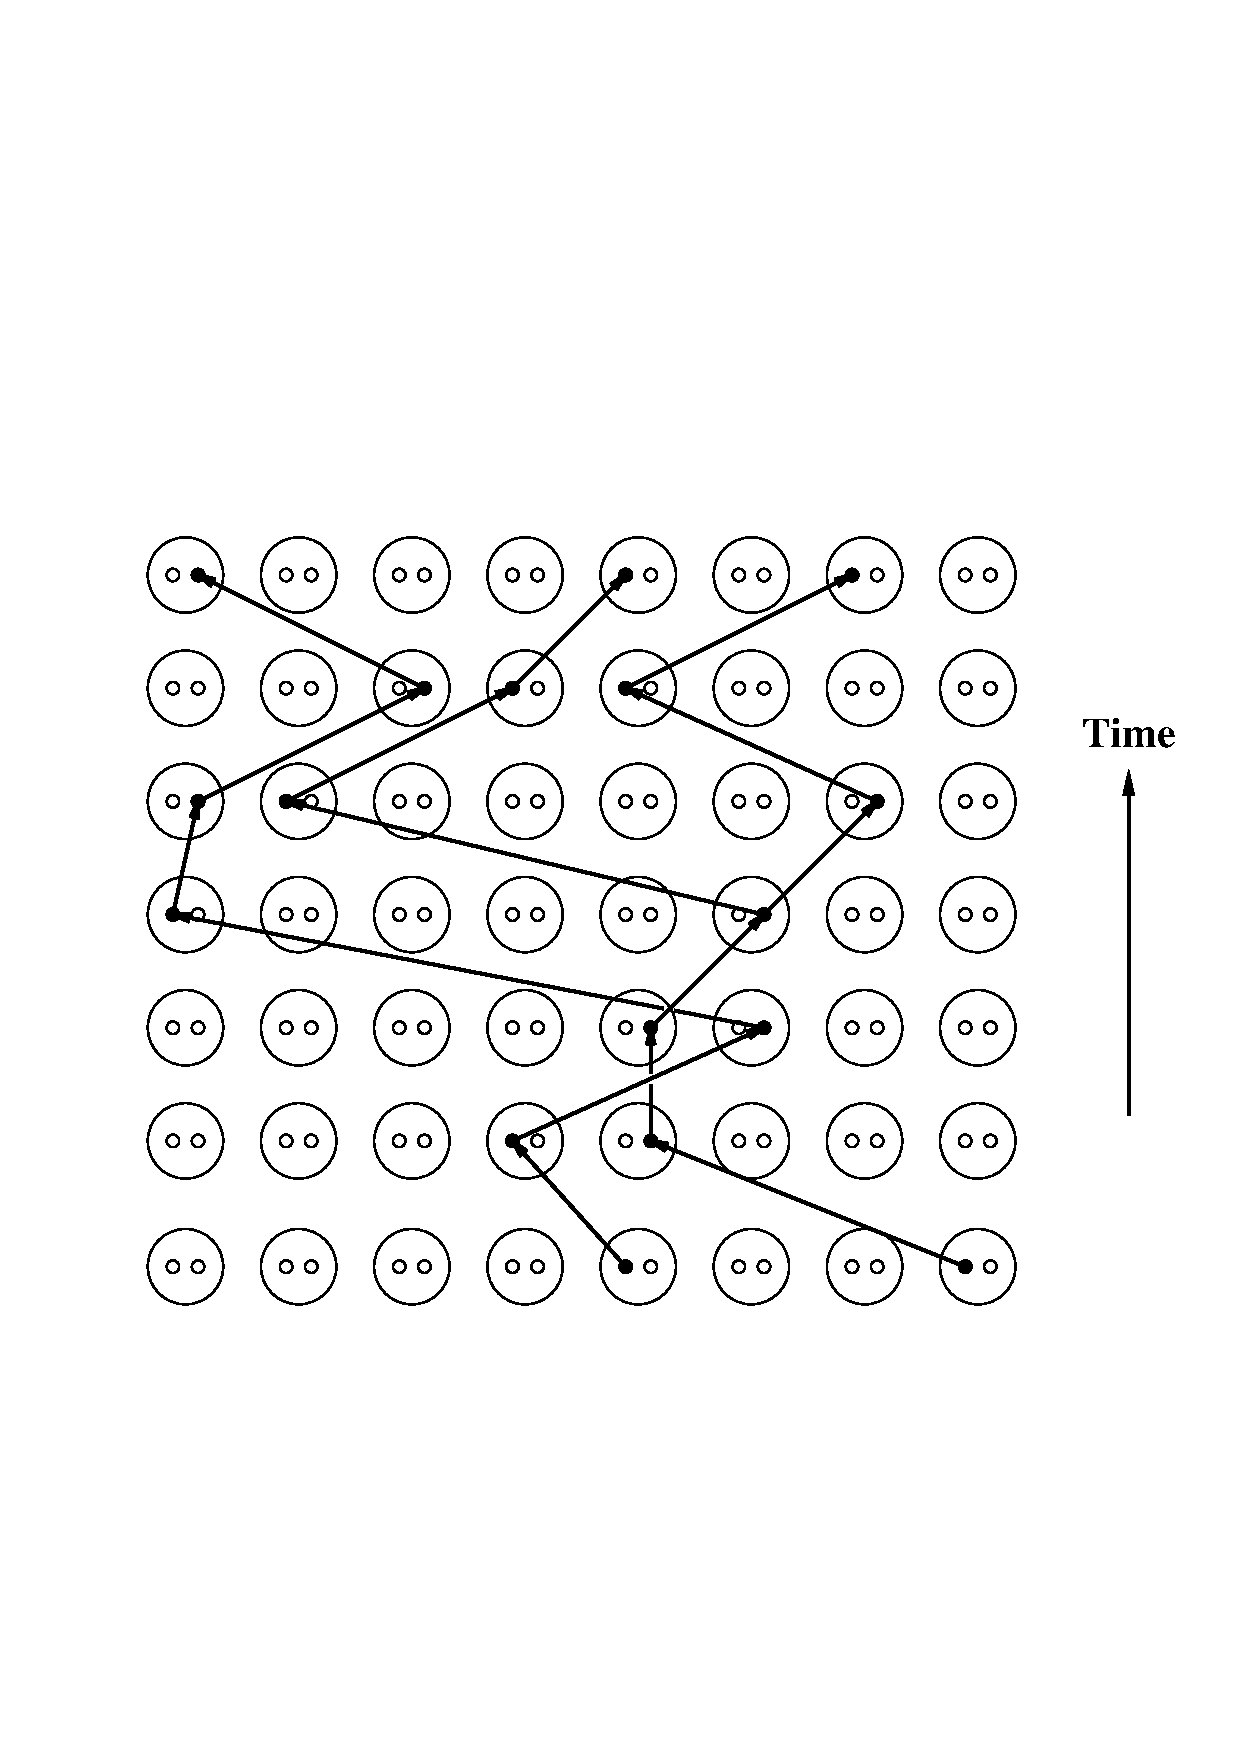
\includegraphics[width=5in]{fig1.pdf}}

\newpage

\centerline{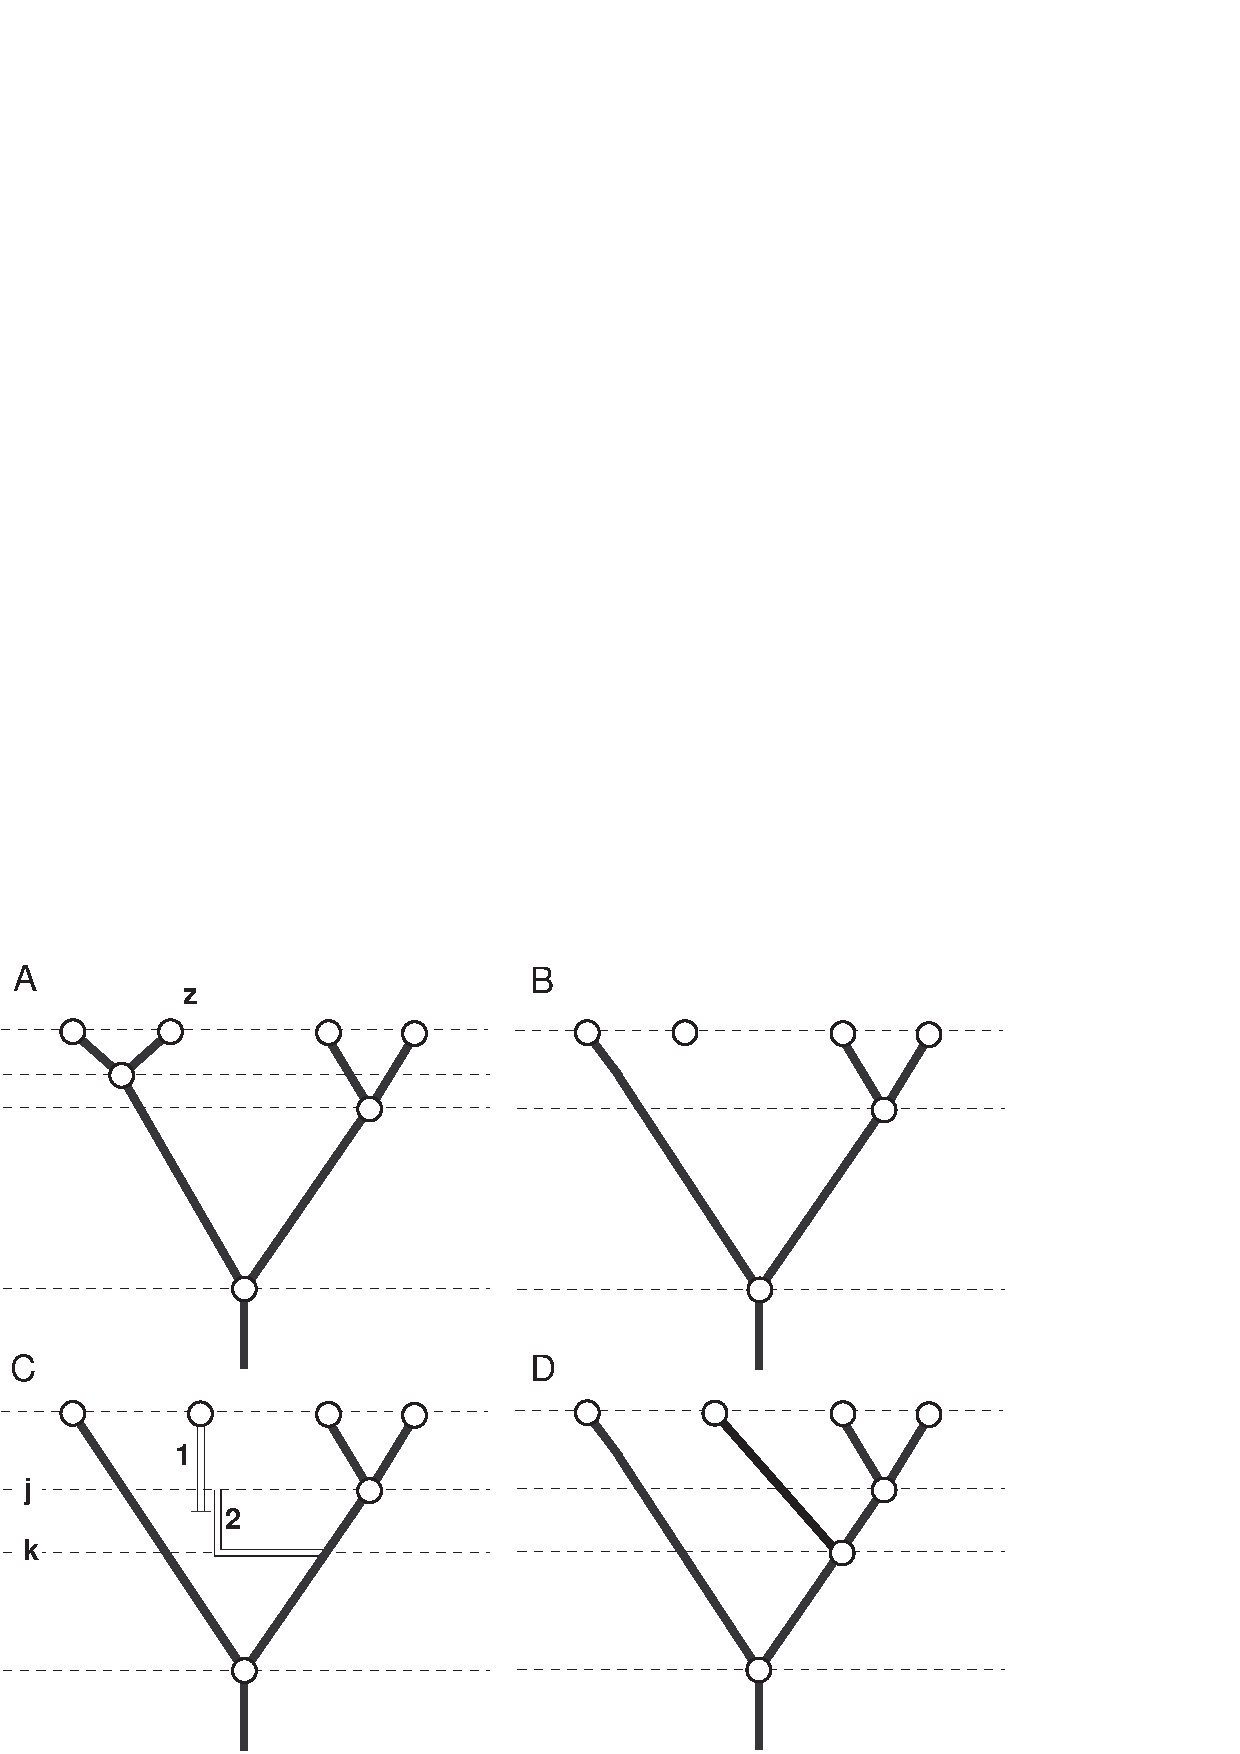
\includegraphics[width=5in]{fig2.pdf}}

\newpage

\centerline{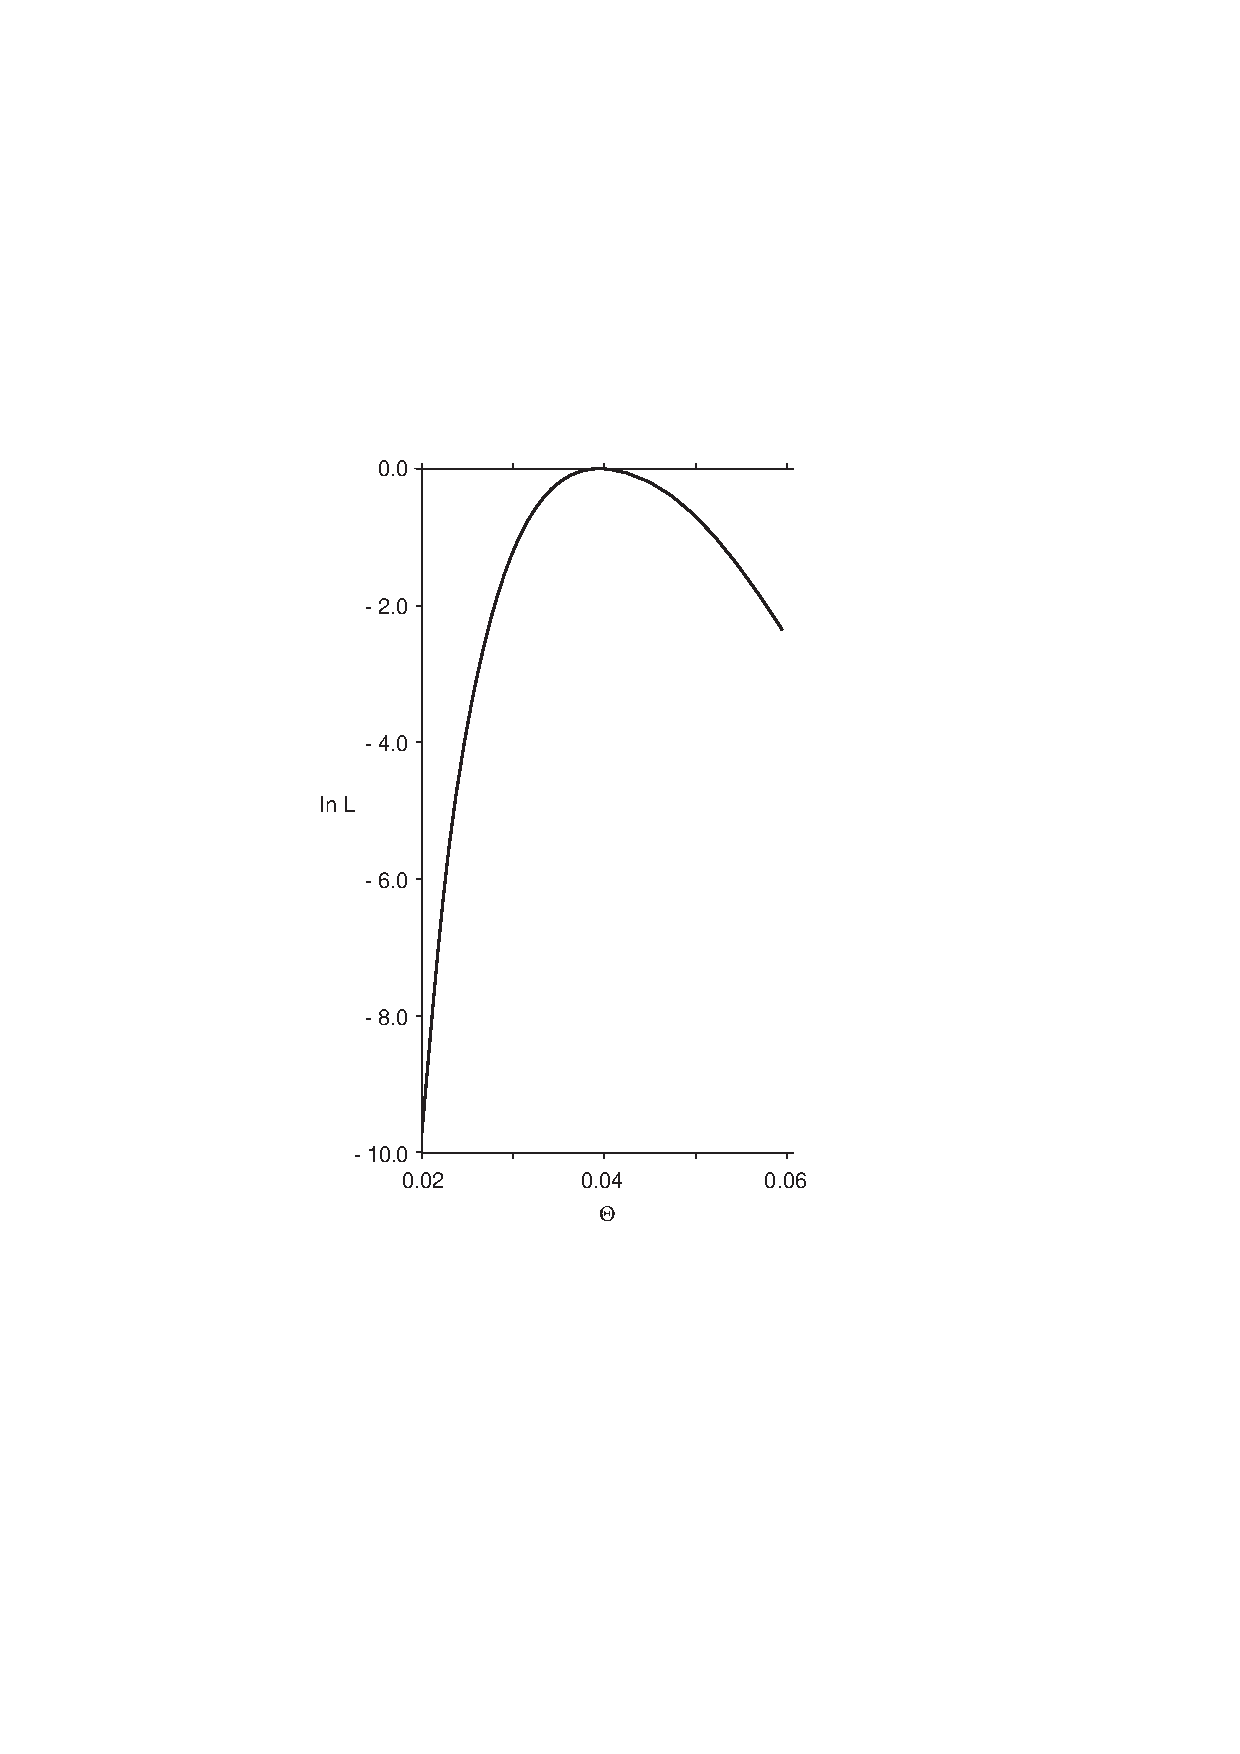
\includegraphics[width=5in]{fig3.pdf}}

\newpage

\centerline{\includegraphics[width=5in]{fig4.pdf}}

\newpage

\centerline{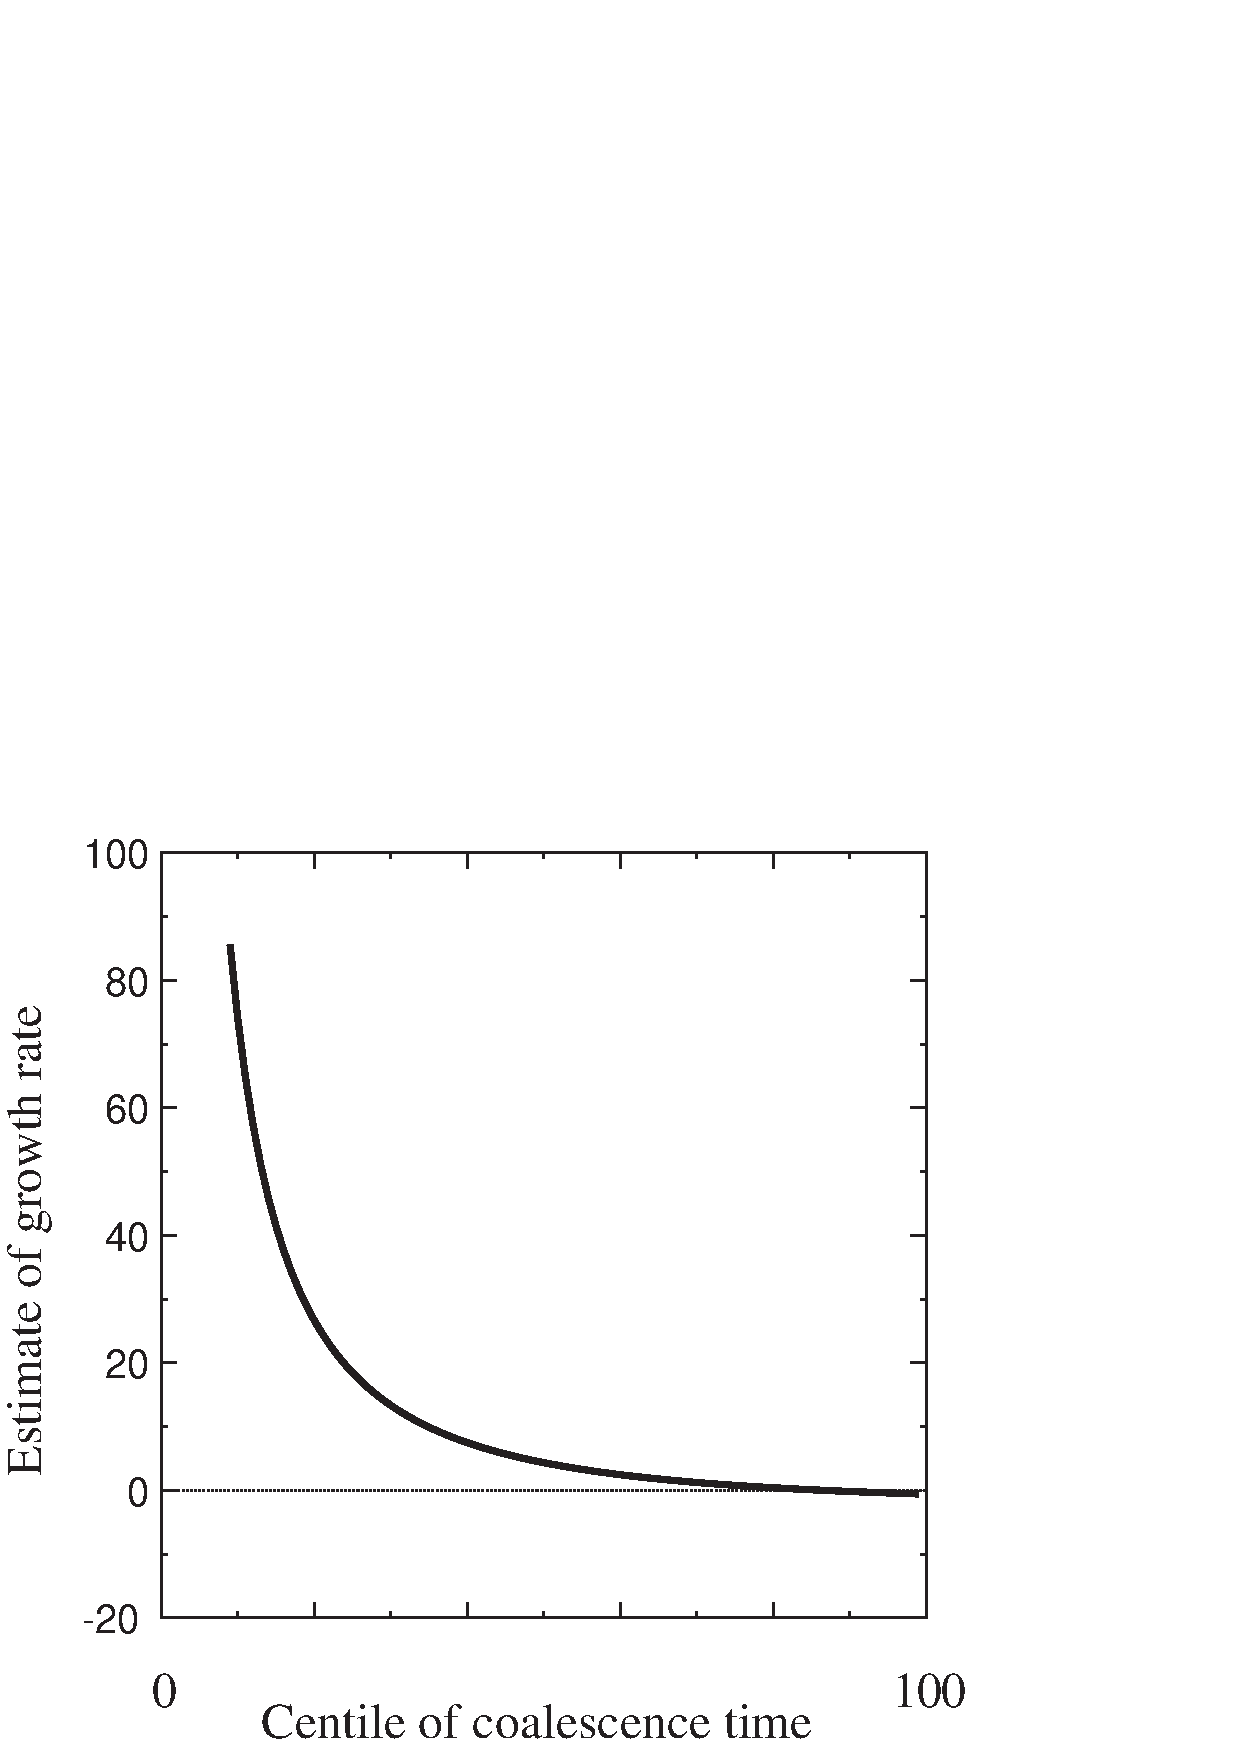
\includegraphics[width=5in]{fig5.pdf}}

\end{document}
